\documentclass[border=3pt,tikz]{standalone}
\usepackage{amsmath}
\usetikzlibrary{calc}
\usetikzlibrary{arrows.meta} % for arrow size
\begin{document}
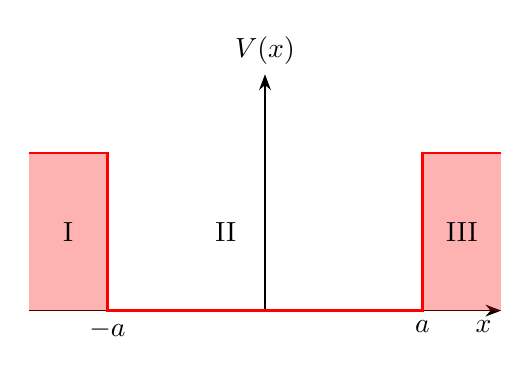
\begin{tikzpicture}[scale=1]
    \draw[, -{Stealth[length=2mm]}] (0, 0) -- (0, 3) node [above] {$V(x)$};
    \draw[, -{Stealth[length=2mm]}] (-3, 0) -- (3, 0) node [below left] {$x$};
    \draw[red, thick, ] (-3, 2) -- (-2, 2) -- (-2, 0) -- (2, 0) -- (2, 2) -- (3, 2);
    \node[below] at (-2, 0) {$-a$};
    \node[below] at (2, 0) {$a$};
    
    \fill [fill=red,fill opacity=0.3] (-2,0) rectangle (-3,2);
    \fill [fill=red,fill opacity=0.3] (2,0) rectangle (3,2);
    
    \node[] at (-2.5, 1) {$\rm{I}$};
    \node[] at (-0.5, 1) {$\rm{II}$};
    \node[] at (2.5, 1) {$\rm{III}$};
    
    \end{tikzpicture}
\end{document}